\documentclass[10pt,landscape]{article}
\usepackage{amssymb,amsmath,amsthm,amsfonts}
\usepackage{multicol,multirow}
\usepackage{calc}
\usepackage{graphicx}
\usepackage{ifthen}
\usepackage[landscape]{geometry}
\usepackage[colorlinks=true,citecolor=blue,linkcolor=blue]{hyperref}


\ifthenelse{\lengthtest { \paperwidth = 11in}}
    { \geometry{top=.5in,left=.5in,right=.5in,bottom=.5in} }
	{\ifthenelse{ \lengthtest{ \paperwidth = 297mm}}
		{\geometry{top=1cm,left=1cm,right=1cm,bottom=1cm} }
		{\geometry{top=1cm,left=1cm,right=1cm,bottom=1cm} }
	}
\pagestyle{empty}
\makeatletter
\renewcommand{\section}{\@startsection{section}{1}{0mm}%
                                {-1ex plus -.5ex minus -.2ex}%
                                {0.5ex plus .2ex}%x
                                {\normalfont\large\bfseries}}
\renewcommand{\subsection}{\@startsection{subsection}{2}{0mm}%
                                {-1explus -.5ex minus -.2ex}%
                                {0.5ex plus .2ex}%
                                {\normalfont\normalsize\bfseries}}
\renewcommand{\subsubsection}{\@startsection{subsubsection}{3}{0mm}%
                                {-1ex plus -.5ex minus -.2ex}%
                                {1ex plus .2ex}%
                                {\normalfont\small\bfseries}}
\makeatother
\setcounter{secnumdepth}{0}
\setlength{\parindent}{0pt}
\setlength{\parskip}{0pt plus 0.5ex}
% -----------------------------------------------------------------------

\title{COMPSCI 2GA3 - Geon}

\begin{document}

\raggedright
\footnotesize

\begin{center}
     \Large{\textbf{COMPSCI 2GA3 - Geon}} \\
\end{center}
\begin{multicols}{3}
\setlength{\premulticols}{1pt}
\setlength{\postmulticols}{1pt}
\setlength{\multicolsep}{3pt}
\setlength{\columnsep}{2pt}

\section{Digital logic}
{\centering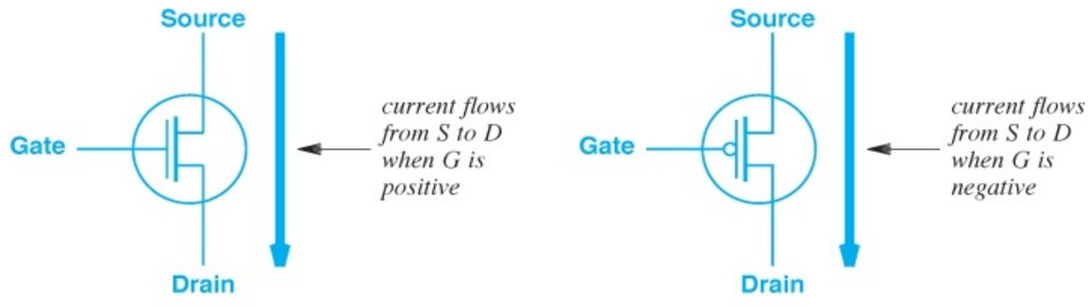
\includegraphics[scale=0.23]{img/trans.png}\par}
{\centering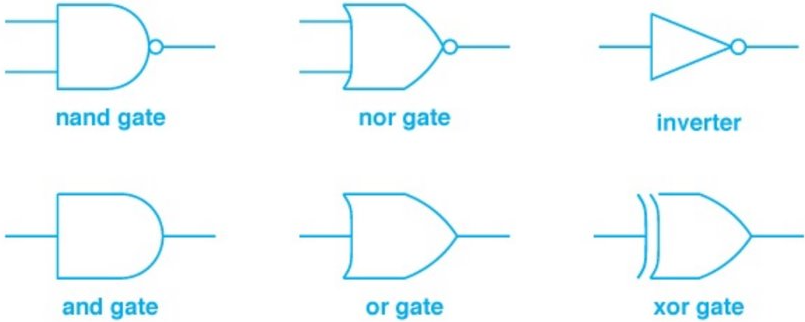
\includegraphics[scale=0.23]{img/lg.png}\par} 
\textbf{Half adder}: takes two input bits, outputs sum (xor) and carry (and).\\
{\centering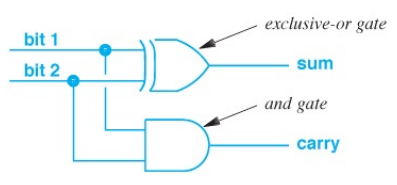
\includegraphics[scale=0.29]{img/had.png}\par} 
\textbf{Full adder}: takes two input bits and a carry, outputs sum and carry. Built from two half adders and an or gate.\\
{\centering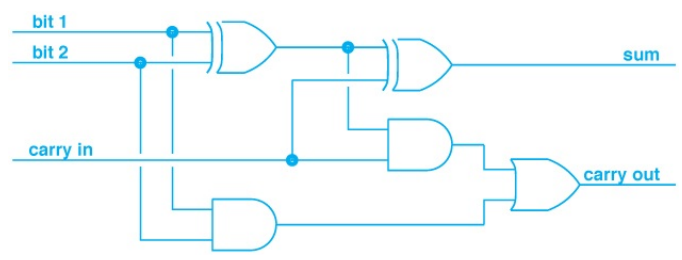
\includegraphics[scale=0.28]{img/fad.png}\par} 
\textbf{Latch}: uses previous output until the enable line is enabled. The output remains the same (even when the enable line is on) until propagation delay is over.\\
{\centering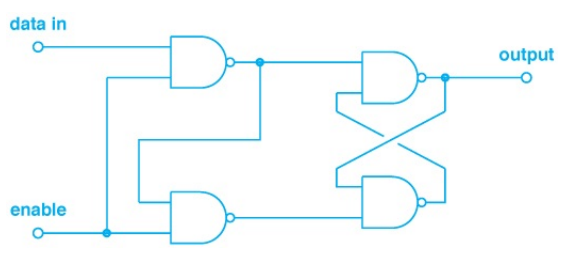
\includegraphics[scale=0.3]{img/l.png}\par}
\textbf{Propagation delay}: the delay between an input change an an output change.\\
\textbf{Register}: stores bits through a series of latches. Different types: general-purpose, floating point, instruction pointer, comparison operation. Use to load data from memory to register, perform ALU operation, and store result from register to memory. \\
{\centering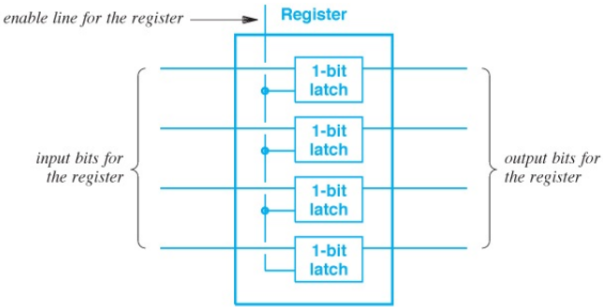
\includegraphics[scale=0.4]{img/register.png}\par}
\textbf{Binary counter}: counts in binary. Takes in 1 input, and with $n$ outputs, it can count from $0$ to $2^n-1$. When the input \textit{goes from 0 to 1}, the counter increments by 1. It can have more inputs for \textit{reset} and \textit{pause}. It can have more outputs for \textit{overflow}.\\
\textbf{Clock}: controls a logic circuit, allowing components to operate without requiring input to change. Oscillates at a regular rate between 1 and 0. \textit{Clocked} components can be synchronized and work as a function of its inputs \textit{and time}.\\
\textbf{Decoder}: takes in a $n$-bit binary value and enables one of $2^n$ outputs.\\
{\centering{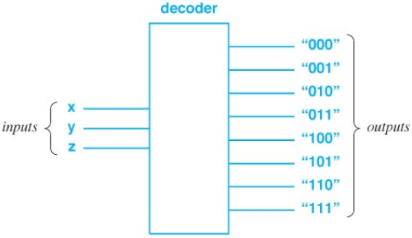
\includegraphics[scale=0.5]{img/decoder.png}}\par}
\textbf{Demultiplexor}: a decoder that takes an extra input which gets passed to the selected output. 
\section{Representations}
\textbf{Bit}: 0 or 1.\\
\textbf{Byte}: group of bits (usually 4).\\
\textbf{Word}: group of bytes (usually 2).\\
\textbf{Big endian}: MSB to LSB (i.e. how we usually read numbers).\\
\textbf{Little endian}: LSB to MSB.\\
\textbf{Integers}:
\begin{enumerate}
\item \textbf{Unsigned}: only positive integers from $0$ to $2^k-1$.
\item \textbf{Sign-magnitude}: MSB is sign, rest is magnitude. From $0$ to $2^{k-1}-1$ and from $-0$ to $-2^{k-1}-1$.
\item \textbf{One's complement}: MSB is sign, rest is magnitude. Flipped for negative. From $0$ to $2^{k-1}-1$ and from $-0$ to $-2^{k-1}-1$.
\item \textbf{Two's complement}: MSB is sign, rest is magnitude. Flipped - 1 for negative. From $0$ to $2^{k-1}-1$ and from $-1$ to $-2^{k-1}$.
\end{enumerate}
\textbf{Floating-point}: 
\begin{enumerate}
\item \textbf{IEEE}: stored as \texttt{sign-exponent-mantissa} (32-bit: 1-8-23, 64-bit: 1-11-52):
$$(-1)^s\cdot(1+m)\cdot 2^{e-b}$$
where $s$ is the sign, $m$ is the mantissa, $e$ is the biased exponent and $b$ is the bias. \\
The exponent is biased so it can have negative numbers while being unsigned:
$$b=2^{k-1}-1$$
where $k$ is the number of bits the exponent has. So,
$$e'=e+b$$
where $e$ is the unbiased exponent. The mantissa is \textit{normalized} and is assumed to start with 1.
\item \textbf{Binary coded decimal}: encode every decimal digit in a byte (4 bits). For fractions, either include an explicit decimal point in the string or specify its location. For signs, a \texttt{0xD} is put at the end to indicate it's negative. 
\end{enumerate}
\section{Processors}
\textbf{Von Neumann architecture}: single memory to hold both instructions and data. More flexible, but bottleneck between memory to processor. More popular than Harvard.\\
{\centering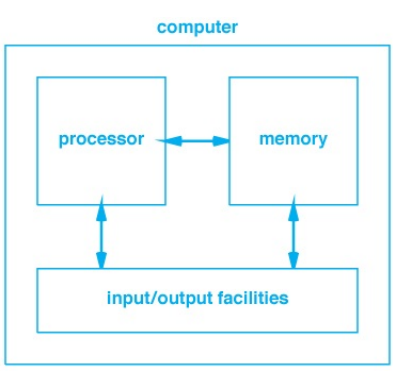
\includegraphics[scale=0.35]{img/vna.png}\par}
\textbf{Harvard architecture}: separate memory for instructions and data. Less susceptible to bottlenecks and more secure, but the split between instructions and data memory is rigid.\\
{\centering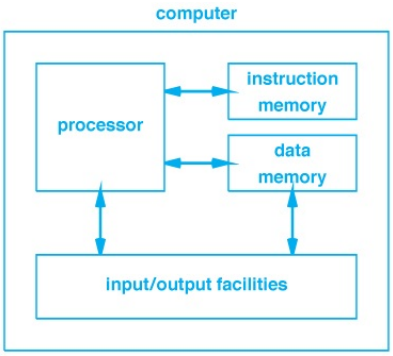
\includegraphics[scale=0.35]{img/ha.png}\par}
\textbf{Processors}: a digital device that can perform multi-step computation.\\
\textbf{Types}:
\begin{enumerate}
\item \textbf{Fixed logic}: function is fixed in hardware.
\item \textbf{Selectable logic}: can choose one of several fixed functions.
\item \textbf{Parameterizable logic}: parameters control computation of fixed functions.
\item \textbf{Programmable logic}: list of instructions provided at runtime.
\end{enumerate}
\textbf{Categories}:
\begin{enumerate}
\item\textbf{Co-processors}: dedicated function; fixed/selectable logic.
\item\textbf{Microcontrollers}: programmable logic, direct hardware control.
\item\textbf{Embedded systems}: real-time OS, dedicated hardware.
\item\textbf{General purpose}: more functionality than embedded systems.
\end{enumerate}
\textbf{Units}:
\begin{enumerate}
\item\textbf{Controller}: controls the flow of program execution.
\item\textbf{Arithmetic logic unit}: performs all computational tasks sequentially according to controller.
\item\textbf{Local storage (registers)}: holds data values.
\item\textbf{Internal connections}: Transfers data values between hardware units (between local storage and ALU).
\item\textbf{External interface}: handles communication between processors and the rest of the computer system.
\end{enumerate}
\subsection{Fetch-execute cycle}
The \textit{instruction pointer} \texttt{ip} automatically moves through the program in memory. The cycle \textit{doesn't proceed at a fixed rate} since execution speed depends on the instruction. The cycle \textit{never ends} (unless the system powers down) so there always needs to be a program executing (either the same program or OS).
\begin{verbatim}
ip = start of program
repeat forever
    instruction = fetch(memory[ip++])
    execute instruction
\end{verbatim}
\subsection{Compilation}
High-level languages are \textit{compiled} into binary \textit{object code} for the processor to compute through the fetch-execute cycle. 
\begin{enumerate}
\item \textbf{Preprocessor}: expands macros.
\item \textbf{Compiler}: translates to assembly language.
\item\textbf{Assembler}: translates to relocatable object code (contains references to external library functions).
\item \textbf{Linker}: replaces external function references with its code.
\end{enumerate}
{\centering 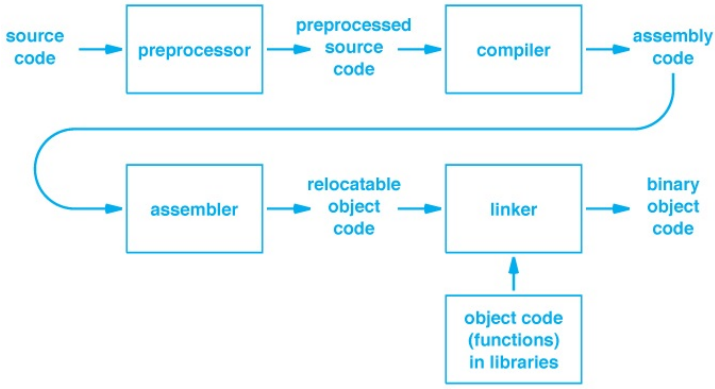
\includegraphics[scale=0.35]{img/c.png}\par}
\section{Instructions}
Usually encoded as \texttt{opcode-operands-offset}.\\
\textbf{Instruction sets}: the \textit{design} of all available instructions for a processor (available instructions, what each instruction does, number of operands, operand encoding, instruction encoding, result storing, etc).\\
\textbf{Branching}: moving the \textit{instruction pointer} to a different location in the program (e.g. for conditionals, loops, etc.).
\begin{verbatim}
ip = start of program
repeat forever
    instruction = fetch(memory[ip])
    tmp = ip + 1
    execute instruction
    ip = tmp
\end{verbatim}
\textbf{Absolute branching}: \texttt{tmp = absolute address}\\
\textbf{Relative branching}: \texttt{tmp = ip + offset}\\
\textbf{Register bank}: each \textit{bank} stores a set of registers. Allows parallel access to different registers within the same clock cycle. Can lead to register bank conflicts if an operation requires multiple registers from the same bank. \\
\textbf{Subroutine}: another word for branching. \\
\textbf{Passing arguments to subroutine calls}: either stored in \textit{memory} or \textit{registers} through \textit{register windows}.\\
\textbf{Register window}: exposing only a set of registers at a time (i.e. a window), which moves each time a subroutine is called and moves back when it returns. The window overlaps with what the program sees and what the subroutine sees so \textit{arguments are passed into the overlapping registers}.\\
{\centering 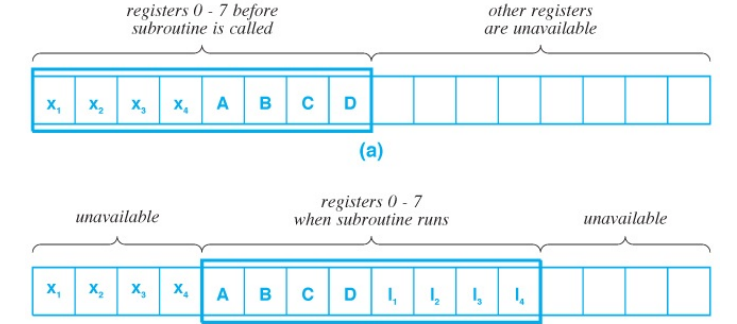
\includegraphics[scale=0.4]{img/rw.png}\par}
\textbf{Complex instruction set computer (CISC)}: a kind of ISA where each instruction performs a \textit{complex operation}, instructions take \textit{variable number} of clock cycles, and requires \textit{fewer instruction calls} than a RISC.\\
\textbf{Reduced instruction set computer (RISC)}:  a kind of ISA where each instruction performs a \textit{simple operation}, instructions take the \textit{same number} of clock cycles (achieved through the RISC pipeline), and requires \textit{many instruction calls}.\\
\textbf{Throughput}: the amount of work done per unit time.\\
\textbf{Pipeline}: a computational architecture that improves throughput if computation can be divided into \textit{distinct stages}, each stage takes \textit{similar time} to complete, and it's \textit{efficient} to move data between stages.\\
\textbf{RISC pipeline}: a 5 stage pipeline for RISC that allows one instruction to execute per clock cycle \textbf{once the pipeline is filled}.\\
{\centering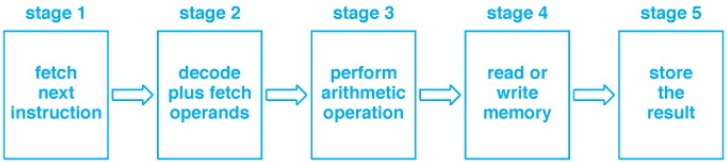
\includegraphics[scale=0.39]{img/rp.png}\par}
\textbf{Stall}: disrupts the flow of a pipeline. Creates a \textit{bubble} that floats until the pipeline restarts. Also called a \textit{hazard}.\\
\textbf{Bubble}: a delay in the pipeline of one or more clock cycles due to a stall.\\
\textbf{Data hazard}: a stall from an instruction \textit{waiting for data} from an earlier instruction. Solved by \textit{forwarding} between stages or \textit{rearranging instructions} so instructions requiring data from earlier instructions occur later. \\
\textbf{Forwarding}: pass results from earlier instructions into later instructions that require it \textit{right after it's calculated} rather than once it's done being stored.\\
\textbf{Control hazard}: a stall from an \textit{incorrect instruction} in the pipeline, causing \textit{branching}. Solved by predicting conditional branching and flushing the pipeline if the prediction is wrong.\\
\textbf{Structural hazard}: a stall from \textit{resource conflicts} where a required resource is needed simultaneously by more than one instruction. Solved by loading data in parallel like in \textit{register banks}.\\
\subsection{Operands}
The arguments of instructions. Can either be \texttt{src} (value, register, address) or \texttt{dst} (register, address).\\
There can be \textit{fixed} (bit fields have same semantics) and \textit{variable} (more memory efficient) number of operands. \\
\begin{enumerate}
\item \textbf{0 operands}: stack architecture.
\item \textbf{1 operands}: implicit destination.
\item \textbf{2 operands}: specified destination, given operand is destination.
\item \textbf{3 operands}: specified destination, can have separate destination from inputs.
\end{enumerate}
\textbf{Implicit encoding}: opcodes define what type of operands we need.\\
\textbf{Explicit encoding}: operand fields define what type of operands.\\
\textbf{Different ways operands can be accessed}:
\begin{enumerate}
\item \textit{Immediate value} in instruction.
\item Value in register, \textit{register id} in instruction.
\item Value in memory, \textit{memory address} in instruction.
\item Value in memory, \textit{memory address in register}, register id in instruction. I.e. pointer.
\item Value in memory, memory address in \textit{different memory location} encoded in instruction. I.e. double pointer.
\end{enumerate}
\end{multicols}
\end{document}
